\setchapterstyle{kao}
\setchapterpreamble[u]{\margintoc}
\chapter{引言}
\labch{intro}

\section{主要思想}

许多现代印刷教科书采用了突出的页边空白处的布局,在这里可以显示小的数字、表格、注释和几乎所有的东西。可以说,这种布局通过将主要文本与辅助材料分离来帮助组织讨论,而辅助材料同时又非常接近文本中引用它的地方。

这份文件的目的并不是要道歉,因为有许多更适合这项任务的作者;所有这些单词的目的只是填充空间,以便读者可以看到用kaobook类编写的书是什么样子的。同时,我还将尝试说明类的特性。

kaobook背后的主要思想来自于这个\href{https://3d.bk.tudelft.nl/ken/en/2016/04/17/a-1.5-column-layout-in latex。html}{blog post},实际上这个类的名称是专门为这篇文章的作者Ken Arroyo Ohori命名的,他允许我根据他的论文创建一个类。因此,如果你想知道更多喜欢1.5栏布局的理由,一定要阅读他的博客文章。

您可能已经注意到,灵感的另一个来源是\href{https://github.com/tuft-latex/tuft-latex}{tuft-latex类}。设计相似的原因是很难改进已经很好的东西。但是,我认为这个类比tuft - latex更灵活。例如,我尝试只使用标准包,并尽可能少地从头实现;\sidenote{这也意味着更容易理解和贡献类开发。实际上,还有很多地方需要改进,所以如果您感兴趣,可以在github上查看存储库!}因此,只要您阅读了提供该特性的包的文档,定制任何东西都应该非常容易。

在本书中,我将阐述该类的主要特性,并提供有关如何使用和更改内容的信息。让我们开始吧。

\section{本类的功能}
\labsec{does}

\Class{kaobook}类更关注文档结构,而不是样式。实际上,众所周知的\LaTeX\xspace 原则是结构和样式应该尽可能地分离(参见\vrefsec{does})。这意味着这个类将只提供命令、环境和一般情况下的机会来执行用户可能使用或不使用的操作。实际上,类中嵌入了一些样式问题,但是用户可以轻松地定制它们。

主要特点如下:

\begin{description}
	\item[Page Layout] 减少文本宽度是为了提高可读性,并为页边距留出空间,以便显示任何类型的元素。
	\item[Chapter Headings] 相对于tuft-latex,我们提供了多种章节标题可供选择;例子将在后面的章节中看到。
	\item[Page Headers] 它们跨越整个页面,包括页边距,并在双侧模式下交替显示章节和节名。\sidenote[-2mm][]{这是Tufte设计的另一个不同之处。}
	\item[Matters] The commands \Command{frontmatter}, 
	\Command{mainmatter} and \Command{backmatter} have been redefined in 
	order to have automatically wide margins in the main matter, and 
	narrow margins in the front and back matters. However, the page 
	style can be changed at any moment, even in the middle of the 
	document.
	\item[Margin text] We provide commands \Command{sidenote} and 
	\Command{marginnote} to put text in the 
	margins.\sidenote[-2mm][]{Sidenotes (like this!) are numbered while 
	marginnotes are not}
	\item[Margin figs/tabs] A couple of useful environments is 
	\Environment{marginfigure} and \Environment{margintable}, which, not 
	surprisingly, allow you to put figures and tables in the margins 
	(\cfr \reffig{marginmonalisa}).
	\item[Margin toc] Finally, since we have wide margins, why don't add 
	a little table of contents in them? See \Command{margintoc} for 
	that.
	\item[Hyperref] \Package{hyperref} is loaded and by default we try 
	to add bookmarks in a sensible way; in particular, the bookmarks 
	levels are automatically reset at \Command{appendix} and 
	\Command{backmatter}. Moreover, we also provide a small package to 
	ease the hyperreferencing of other parts of the text.
	\item[Bibliography] We want the reader to be able to know what has 
	been cited without having to go to the end of the document every 
	time, so citations go in the margins as well as at the end, as in 
	Tufte-Latex. Unlike that class, however, you are free to customise 
	the citations as you wish.
\end{description}

\begin{marginfigure}[-5.5cm]
	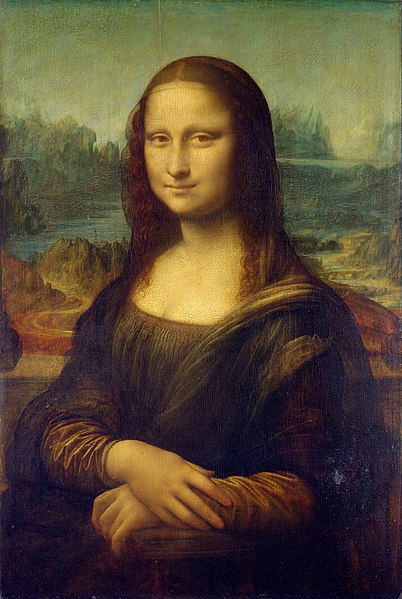
\includegraphics{monalisa}
	\caption[The Mona Lisa]{The Mona Lisa.\\ 
	\url{https://commons.wikimedia.org/wiki/File:Mona_Lisa,_by_Leonardo_da_Vinci,_from_C2RMF_retouched.jpg}}
	\labfig{marginmonalisa}
\end{marginfigure}

The order of the title pages, table of contents and preface can be 
easily changed, as in aly \LaTeX\ document. In addition, the class is 
based on \KOMAScript's \Class{scrbook}, therefore it inherits all the 
goodies of that.

\section{本类未实现的功能}
\labsec{doesnot}

As anticipated, further customisation of the book is left to the user. 
Indeed, every book may have sidenotes, margin figures and so on, but 
each book will have its own fonts, toc style, special environments and 
so on. For this reason, in addition to the class, we provide only 
sensible defaults, but if these features are not nedded, they can be 
left out. These special packages are located in the \Path{style} 
directory, which is organised as follows:

\begin{description}
	\item[style.sty] 这个包包含页面布局、页眉和页脚、章节标题和整个文档中使用的字体的规范。
	\item[packages.sty] 加载额外的包,用特殊的内容来装饰写作(例如,这里加载\Package{listing}包,因为不是每本书都需要它)。还定义了一些有用的命令,用于以相同的方式打印相同的单词,例如斜体的拉丁单词或逐字的\Package{packages}。
	\item[references.sty] 一些有用的命令来管理标签和引用,再次确保以一致的方式引用相同的元素。
	\item[environments.sty] 提供特殊的环境,比如框。简单和复杂的环境都是可用的;所谓复杂,我们的意思是它们被赋予一个计数器,浮动的,可以放在一个特殊的目录中。\sidenote[-2mm][]{参考 
	\vrefch{mathematics}来获取更多示例。}
	\item[theorems.sty] The style of mathematical environments. 
	Acutally, there are two such packages: one is for plain theorems, 
	\ie the theorems are printed in plain text; the other uses 
	\Package{mdframed} to draw a box around theorems. You can plug the 
	most appropriate style into its document.
\end{description}

\marginnote[2mm]{The audacious users might feel tempted to edit some of 
these packages. I'd be immensely happy if they sent me examples of what 
they have been able to do!}

In the rest of the book, I shall assume that the reader is not a novice 
in the use of \LaTeX, and refer to the documentation of the packages 
used in this class for things that are already explained there. 
Moreover, I assume that the reader is willing to make minor edits to the 
provided packages for styles, environments and commands, if he or she 
does not like the default settings.
